\documentclass[11pt]{article}
\usepackage[a4paper, margin=3cm]{geometry}


\usepackage[T1]{fontenc}
\usepackage[utf8]{inputenc}
\usepackage{lmodern}

\usepackage[english]{babel}
\usepackage{microtype}

\usepackage{graphicx}
\usepackage{hyperref}
\usepackage{amsmath,amsfonts,amssymb,amsthm}
\usepackage{color}
\usepackage{listings}


\newcommand{\N}{\ensuremath{\mathbb{N}}}
\newcommand{\Z}{\ensuremath{\mathbb{Z}}}
\newcommand{\Q}{\ensuremath{\mathbb{Q}}}
\newcommand{\R}{\ensuremath{\mathbb{R}}}



\graphicspath{{img/}}



\title{\vspace{-8ex}
\huge Rays-Crashing\\
{\normalsize Project Report}}

\author{Etienne Moutot [\href{mailto:etienne.moutot@ens-lyon.org}{etienne.moutot@ens-lyon.org}]}
\date{08/01/2017}

\begin{document}

\maketitle

\begin{figure}[h]
\centering
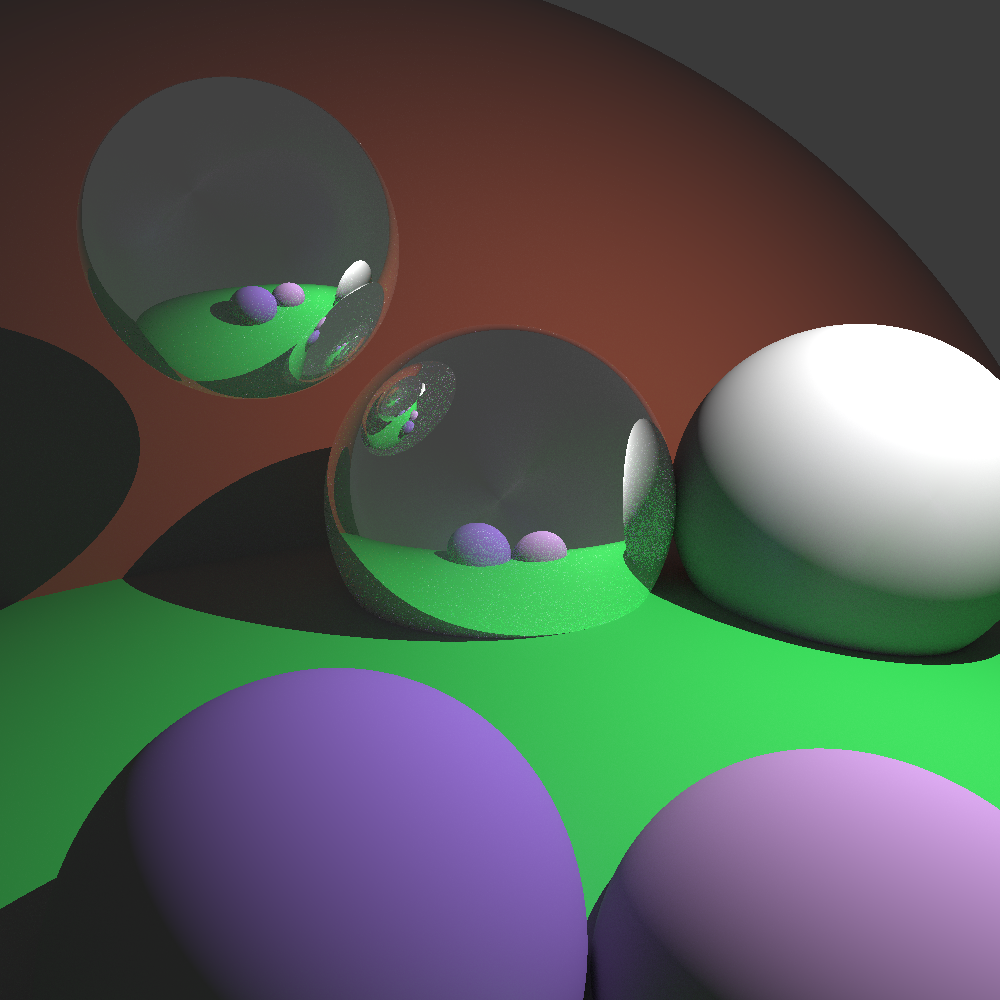
\includegraphics[width=10cm]{img/ex_1000.png}
\end{figure}

\section{Presentation}
Rays-crashing is a basic raytracer which is able to render only scenes containing spheres at the moment. It has the following features:
\begin{itemize}
  \item Direct illumination
  \item Materials: Diffuse, Specular and Transparent
  \item Indirect illumination using Monte-Carlo method
  \item Parallelization
  \item Gamma correction
\end{itemize}

\section{Using Rays-Crashing}
To build the project, you can clone it from github: \texttt{https://github.com/coma94/rays-crashing.git}
Then build and lunch it:
\begin{lstlisting}[language=bash]
  cmake .
  make
  ./rays-crashing
\end{lstlisting}
The dependencies are only OpenMP.

For the moment the scene is generated in src/main.ccp. You need to rebuild rays-crashing every time you change the scene.

The rendering parameter are also build in the main. To change the size of the output image, change the 1000, 1000 at line 59:
\begin{center}
	\begin{lstlisting}[language=c++]
	Camera cam = Camera(Vector3(0,0,20), 1.05, 1000, 1000);
	\end{lstlisting}
\end{center}
For the filename of the rendered file and the number of rays lunched for the indirect lightning, see line 65:
\begin{center}
	\begin{lstlisting}[language=c++]
	cam.render("bla.png", 100);
	\end{lstlisting}
\end{center}

\section{Code Organization}
The directory \texttt{include/} contains the C++ headers and \texttt{src/} the sources files. Several classes are defined and used in this project:
\begin{description}
  \item[Image] (image.h/cpp): C++ layer over CIming, to store images in memory and save them.
  \item[Vector3] : 3-dimensional vector with double coordinates, and a lot of operation between them (addition, products, norm, ...).
  \item[Material] (objects.h/cpp): Contains properties of the material of objects.
  \item[Ray] : A ray. Contains a method ton compute its intersection with a sphere.
  \item[Sphere] (objects.h/cpp): A sphere of the scene with a material. Contains a method ton compute its intersection with a ray.
  \item[Light] (objects.h/cpp): Contains properties of the light of the scene.
  \item[Scene] (objects.h/cpp): The scene itself, containing objects, a light and a method to compute the value of a point seen by a specific ray.
  \item[Camera] (objects.h/cpp): The camera, given a scene it renders it into a png file.
\end{description}


\end{document}
